\begin{exercise}
      {ID-8cc6fac3aac6467dd0a9346cb776e9a3c199a3db}
      {Grundstück}
  \ifproblem\problem\par
    % <PROBLEM>
    \begin{minipage}[c]{0.38\textwidth}
      \centering
      \begin{tikzpicture}[scale=0.32, line width=0.6pt]
        % default colors
        \newcommand{\colr}{Red};%
        \newcommand{\colg}{ForestGreen};%
        \newcommand{\colb}{Cerulean};%
        \newcommand{\coly}{YellowOrange};%
        \newcommand{\cola}{Black!35!White};%
        \newcommand{\cole}{Black!55!White};%
        \coordinate (A) at ( 0.00, 0.00);
        \coordinate (B) at (11.25, 0.00);
        \coordinate (C) at ( 7.50, 7.29);
        \coordinate (D) at ( 0.00, 7.29);
        \draw[fill=\cola] (A) -- (B) -- (C) -- (D) -- cycle;
        \path (A) -- node[below] {\small\simeter{112.5}} (B);
        \path (C) -- node[above] {\small\simeter{75}} (D);
        \path (B) -- node[shift=(27.5:3mm), rotate=-62.5] {\small\simeter{62.5}} (C);
      \end{tikzpicture}
    \end{minipage}\hfill
    \begin{minipage}[c]{0.6\textwidth}
      Ein trapezförmiges Grundstück soll verkauft werden. Der Eigentümer verlangt
      \eur{32} für einen Quadratmeter. Wie teuer ist das gesamte Grundstück?
    \end{minipage}
    % </PROBLEM>
  \fi
  %\ifoutline\outline\par
    % <OUTLINE>
    % </OUTLINE>
  %\fi
  \ifoutcome\outcome\par
    % <OUTCOME>
    Sobald man den Abstand $h$ der parallelen
    Grundstücksgrenzen kennt, kann man den
    Flächeninhalt des trapezförmigen Grundstücks berechnen:
    \begin{center}
      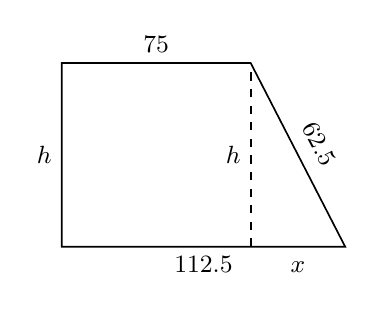
\begin{tikzpicture}[scale=0.32, line width=0.6pt]
        \coordinate (A) at ( 0.00, 0.00);
        \coordinate (B) at (11.25, 0.00);
        \coordinate (C) at ( 7.50, 7.29);
        \coordinate (D) at ( 0.00, 7.29);
        \coordinate (H) at ( 7.50, 0.00);
        \draw (A) -- (B) -- (C) -- (D) -- cycle;
        \path (A) -- node[below] {\small\simeter{112.5}} (B);
        \path (C) -- node[above] {\small\simeter{75}} (D);
        \path (B) -- node[shift=(27.5:3mm), rotate=-62.5] {\small\simeter{62.5}} (C);
        % h
        \draw[style=dashed] (H) -- node[left]{\small$h$} (C);
        \path (D) -- node[left] {\small$h$} (A);
        % x
        \path (H) -- node[below] {\small$\vphantom{8}x$} (B);
      \end{tikzpicture}
    \end{center}
    Der Abstand $h$ lässt sich mithilfe des Satzes
    des Pythagoras ermitteln, denn es gilt:
    \begin{equation*}
      h^2+x^2=\num{62.5}^2\text{\,\si{\square\metre}}
      \quad\Rightarrow\quad
      h=\sqrt{\num{62.5}^2-x^2}\text{\,\si{\metre}}
    \end{equation*}
    Die Länge der Strecke $x$ entspricht der Differenz
    der beiden parallelen Grundstücksgrenzen:
    \begin{equation*}
      x=\SI{112.5}{\metre}-\SI{75}{\metre}=\SI{37.5}{\metre}
    \end{equation*}
    Damit kann man jetzt den Abstand $h$ berechnen:
    \begin{equation*}
      h=\sqrt{\num{62.5}^2-\num{37.5}^2}\text{\,\si{\metre}}
       =\SI{50}{\metre}
    \end{equation*}
    Für den Flächeninhalt $A$ ergibt sich nun:
    \begin{equation*}
      A=\frac{\SI{112.5}{\metre}+\SI{75}{\metre}}{2}\cdot\SI{50}{\metre}
      =\SI{4687.5}{\square\metre}
      %(112.5 + 75)/2 * 50
    \end{equation*}
    Wenn der Eigentümer \eur{32} pro Quadratmeter
    verlangt, dann muss man für das gesamte Grundstück
    genau \eur{150000} zahlen.
    %(112.5 + 75)/2 * 50 * 32
    % </OUTCOME>
  \fi
\end{exercise}
